% Document
\documentclass[12pt, a4paper]{article}
\usepackage[T1]{fontenc}
\usepackage[utf8]{inputenc}
\usepackage{authblk}
\usepackage{lipsum}

% Fig. and table formating
\usepackage{epsfig}
\usepackage{tabu}
\usepackage{rotating}
\usepackage{pbox}
\usepackage{framed, multicol}
\usepackage[framemethod=TikZ]{mdframed}
\usepackage{float}
\usepackage[left=1.25 in, right=1.25 in, top=1.25 in, bottom=1.25 in]{geometry}

\usepackage{caption}

% Fonts - Mathtime
%\usepackage{txfonts}
\usepackage{amsmath} % Add amssymb if not using Mathtime
\newcommand\numberthis{\addtocounter{equation}{1}\tag{\theequation}}

% Text
\setlength{\parindent}{0.5in}
\frenchspacing  \tolerance = 800  \hyphenpenalty = 800

\usepackage{lineno} % Line numbers
\def\linenumberfont{\normalfont\footnotesize\ttfamily}
\setlength\linenumbersep{0.2 in}

\usepackage{setspace}

% Format section and subsection headers
\makeatletter
\renewcommand{\section}{\@startsection
{section}%                   % the name
{1}%                         % the level
{0mm}%                       % the indent
{-\baselineskip}%            % the before skip
{0.5\baselineskip}%          % the after skip
{\normalfont\bf\large}} % the style

\renewcommand{\subsection}{\@startsection
{subsection}%                   % the name
{2}%                         % the level
{0mm}%                       % the indent
{-\baselineskip}%            % the before skip
{0.5\baselineskip}%          % the after skip
{\normalfont\bf}} % the style
\makeatother

% Other
\usepackage{graphicx}
\usepackage[singlelinecheck=false,font=small,labelfont=bf]{caption}
\usepackage[justification=centering]{caption}

% Bibliography
\usepackage[numbers, compress]{natbib} % Bibliography - APA
\bibpunct{(}{)}{;}{a}{}{,}

% Format the Bibliography appropriately
% increase \bibhang to take care of the numbers
\setlength{\bibhang}{0pc}
\makeatletter
%patch \@lbibitem to print the current number before the authors
\patchcmd{\@lbibitem}
  {]}
  {] \theNAT@ctr. \newline }
  {}{}
\makeatother


%%%%%% FRONT MATTER %%%%%%%%%

\title{Comparing methods for estimating parasite-induced host mortality from distributional data: implementation and limitations}
\author{Mark Wilber, Sara Weinstein, and Cherie Briggs}


\begin{document}


\maketitle

\section*{Abstract}

TODO

\doublespacing

\linenumbers
\section*{Introduction}

Infectious agents can have major impacts on animal populations
through changing population dynamics and stability \citep{Dobson1992}, altering
predator-prey interactions \citep{Joly2004}, and even causing species decline
and extinction \citep{DeCastro2005a,McCallum2012b}. Accurate estimates of
parasite-induced host mortality (PIHM) in wild animals are important for
understanding what regulates both host and parasite populations and to make
predictions about disease transmission in natural systems. Although a negative
impact on host fitness is a fundamental component of parasitism
\citep{Lafferty2002} [more], it is notoriously difficult to quantify PIHM in
wild animal populations \citep{Lester1984,McCallum2000a}.

To conclusively identify PIHM in wild animal populations, it is necessary to
experimentally infect and track host populations; a method that is rarely
possible in most wild animal systems \citep{McCallum2000a}.  Instead, parasitologists
are often only able to determine the parasite intensity on some number of sampled hosts.  This snapshot, distributional data is far from the
ideal type of data for addressing questions regarding PIHM, but this is the type of data on which most questions regarding PIHM are asked \citep{Ferguson2011,Royce1990,Lanciani1989,Lester1984,Lester1977}.  In particular, parasitologists are often interested in asking two questions from this data: 1) Is PIHM occurring in a host-parasite system? and if PIHM is occurring 2) Can the effect of parasite intensity on host survival be quantified? While both macro and
microparasites have detrimental and possibly fatal effects on hosts, for the
remainder of this paper we limit our discussion to macroparasites that can be
discretely counted within a host.

The first of these PIHM questions was addressed by \cite{Crofton1971a} who developed
a method to test for the presence of PIHM using the truncation of the negative binomial
distribution.  In short, the Crofton Method assumes that the distribution of
parasites across hosts before mortality occurs follows a negative binomial
distribution \citep{AndersonandMay1978,Shaw1998}.  As heavily infected hosts
begin to die, the negative binomial distribution is truncated and these hosts are no longer observed in a sample. In other words, the
observed host-parasite distribution and the pre-mortality host-parasite
distribution will predict substantially different numbers of hosts with high infect intensity (because those have died due to infection), but a similar number of hosts with low infection
intensity (because those have survived).  \cite{Crofton1971a} noted that by
starting with all observed hosts and iteratively fitting a negative binomial
distribution to hosts with lower and lower parasite loads, one could determine
whether or not PIHM was occurring and estimate the parameters of the host distribution before parasite-induced mortality.  This was done
graphically by determining whether the parameters of the negative binomial distributions fit to different truncations of the data showed a substantial change as the truncation point moved from heavily infected hosts to lightly infected hosts.  The Crofton Method and this graphical technique are both still currently used to assess whether PIHM is a occurring in a system \citep{Ferguson2011}. We give a thorough description and implementation of the Crofton Method in \emph{Supplementary Information} (SI) 1 and discuss the validity of its assumptions in the \emph{Discussion}.

The second question regarding PIHM moves beyond a simple yes or no answer and attempts to quantify how parasite intensity affects host survival. \cite{Adjei1986} proposed a method to answer this question
by first using the Crofton Method to estimate the pre-mortality parameters for
a host-parasite distribution and then, given these
parameters, estimating a host survival function that described how the
probability of host-survival changed with increasing parasite load (see
\emph{Methods}).  With this host survival function, one can estimate important host-parasite quantities such as the
parasite intensity at which 50\% of hosts succumb to PIHM ($LD_{50}$), as well
as the percent of hosts in a population succumbing to PIHM \citep{Adjei1986}.

Despite these methods both being over three decades old, they are still the
primary means of answering questions about PIHM given distributional data
\citep[but see][for an alternative to the Crofton
Method]{Ferguson2011}. However, both methods have a few important limitations.
The Crofton Method, and more recent methods \citep{Ferguson2011},
rely on a visual test to determine whether or not PIHM is occurring in a
system.  With no clear decision rule, it can be difficult to consistently determine the
significance of PIHM across different host-parasite systems. In theory, the Adjei Method can ameliorate this problem. In addition to providing information on the host-survival function, this method can also be used to assess the significance of
PIHM in a system.
In practice, however, the Adjei Method has never been thoroughly tested and
relies on a number of questionable data manipulations.

In this study, we have
three primary goals. First we wish to test reliability of the Adjei Method for
answering the aforementioned questions regarding PIHM.  Second, we propose a
novel method for answering these questions, compare its efficacy against the Adjei Method, and test both methods ability to detect PIHM on empirical data.  Third, we
discuss the limitations of inferring PIHM from distributional data alone and
whether any method for inferring PIHM has a place in the future of
parasitology.

\section*{Methods}

\subsection*{The Adjei Method for estimating PIHM}

The Adjei Method for estimating PIHM has two steps.  The first
step is to estimate the parameters of the pre-mortality host-parasite
distribution using the Crofton Method.  The three parameters estimated are the
total number of hosts before mortality $N_p$,  the mean number of parasites per
host before mortality $\mu_p$, and the aggregation of parasites before
mortality given by the parameter $k_p$ from a negative binomial distribution.
When $k_p$ is small, parasites are highly aggregated among hosts and when
$k_p$ is large parasites are more evenly spread out \citep{Wilson2002}.  The implementation of the Crofton Method has been discussed at length elsewhere \citep[e.g.][]{Royce1990,Lester1984} and we provide a tested implementation of the method in SI 3.

The second step of the Adjei Method is to estimate the shape of the host survival function. \cite{Adjei1986} assume that the host survival function follows the logistic form

\begin{equation}
    h(x | a, b) = h_x = \dfrac{e^{a - b \log(x)}}{1 + e^{a - b \log(x)}}
    \label{eq:logistic}
\end{equation}
where $x$ is the parasite intensity in a given host and $a$ and $b$ are the two
parameters of the logistic function. Generally, a larger $a$ allows for hosts to
tolerate larger parasite intensities before experiencing parasite-induced mortality
and a larger $b$ leads to a more rapid decline in the probability of host
survival as parasite intensity increases.  The value $\exp(a / b)$ is referred
to as the $LD_{50}$, which gives the parasite intensity at which 50\% of hosts
experience mortality.

To estimate this function the Adjei Method proceeds as follows.  First, it
calculates the expected number of hosts with a given parasite load $x$ by using
the equation $g(x ; \mu_p, k_p) * N_p$ where $g(x ; \cdot)$ is the negative binomial pre-mortality distribution.  Second, the observed and predicted number of hosts
with $x$ parasites are paired as a single data point and the method then assumes that
this data point follows a binomial distribution with the total number of
``trials'' equal to the predicted number of hosts and the total number of
``successes'' equal to the observed number of hosts. In some cases, the
observed number of hosts is greater than the expected number of hosts and the
Adjei Method alters the data so that the observed is equal to the predicted
\citep{Adjei1986}.  After this questionable manipulation, the (observed, predicted) pairs are fit to a standard Generalized Linear Model \citep{McCullagh1989} with a binomial response variable and a logistic link function given by equation \ref{eq:logistic}.  This model provides estimates for parameters $a$, $b$ and $LD_{50}$.

While not included in the original implementation of the Adjei Method, a
$\chi^2$ test with a degrees of freedom of 1 can be used to assess whether a GLM model that includes parasite
intensity as a predictor of host survival probability is a ``better'' model than a
GLM without this predictor.  This allows the Adjei Method to determine whether
PIHM is a significant factor in a host-parasite system.

The Adjei Method's most glaring deficiency is the need to alter the observed
data in order to fit the model into the binomial GLM framework.  A second more
subtle problem with the Adjei Method is the potential need to bin data in order
to predict greater than one host in a given parasite intensity class.  For
example, if the total number of hosts pre-mortality was 50, the mean number of
parasites per host pre-mortality was 100 and the aggregation parameter was 1, applying the equation $g(x ; \mu_p=100, k_p=1) * 50$ would result in
less than 1 individual in all parasite intensities $x$. In other words, the
Adjei Method cannot be applied to samples with either very high mean parasite
loads, small sample sizes, or both without some sort of binning of the data.
While this is not a flaw \emph{per se}, it does add a certain level of
subjectivity (i.e. which bins should you use?) to a method that already has
serious potential issues.  In this analysis, we always assume the Adjei Method is not binning the data, though we provide code for applying the binning method in SI 3.

\subsection*{The Likelihood Method for estimating PIHM}

Given the potential deficiencies of the Adjei Method, we provide an alternative
approach for estimating parasite-induced host mortality (PIHM) that makes less
assumptions and provides more reliable answers to the PIHM questions outlined above.  The Likelihood Method we propose
does not require any binning or alteration of the data, potentially reduces the
number of parameters that need to be estimated, and allows for standard
statistical techniques to be used to assess the significance of PIHM in a
system.

As with all previously proposed methods for estimating PIHM, the
Likelihood Method first assumes that the pre-mortality distribution follows a
negative binomial distribution $g(x; \mu_p, k_p)$.  The second
assumption is that the host survival function
takes the form of a logistic curve given by equation \ref{eq:logistic}.  With these two explicit assumptions, the Likelihood Method estimates the 4 parameters $\mu_p$, $k_p$, $a$, and $b$.

To estimate these parameters, we need to define a probability distribution that gives the probability of having a parasite load of $x$ parasites conditional on host survival.  Using standard rules of conditional probability this distribution can be written as

\begin{equation}
    P(x | \text{survival}) = \dfrac{P(\text{survival} | x) * P(x)}{P(\text{survival})}
    \label{eq:concept}
\end{equation}

One can see that $P(\text{survival} | x)$ is the survival function $h(x; a, b)$, $P(x)$ is the pre-mortality parasite distribution $g(x; \mu_p, k_p)$ and $P(\text{survival}) = \sum_0^{\infty} P(\text{survival} | x) * P(x) =  \sum_{x=0}^{\infty} h(x; a, b)  * g(x; \mu_p, k_p)$. Therefore equation \ref{eq:concept} can be written as

\begin{equation}
    P(x | \text{survival}) = \dfrac{h(x; a, b)  * g(x; \mu_p, k_p)}{\sum_{x=0}^{\infty} h(x; a, b)  * g(x; \mu_p, k_p)}
    \label{eq:dist}
\end{equation}

Using this probability distribution, one can then find the parameters $\mu_p$, $k_p$, $a$, and $b$ that maximize the likelihood of an observed host-parasite dataset. Alternatively, one could apply the Crofton Method to estimate $\mu_p$ and $k_p$ and then find the maximum likelihood estimates of $a$ and $b$ and the corresponding $LD_{50}$.

To estimate that significance of PIHM in a host-parasite system, a
likelihood ratio test can be used in which the full model is given by equation
\ref{eq:dist} and the reduced model is given by a negative binomial
distribution.  If PIHM is not significant in the system, the resulting likelihood
ratio statistic should approximately follow a $\chi^2$ distribution with degrees of freedom equal to 2.  We provide the code for implementing this Likelihood Method in SI 3.

\subsection*{Question 1: Is PIHM occurring?}

To test the ability of the Adjei Method and the Likelihood Method to identify whether or not PIHM was occurring in a system, we randomly generated data using the following procedure.  First, we drew $N_p$ randomly infected hosts from a
negative binomial distribution with parameters $\mu_p$ and $k_p$.  This represented the dataset observed before mortality. Second, we chose values of $a$ and $b$ and calculated the probability of survival
for all $N_p$ hosts using equation \ref{eq:logistic}.  Third, we drew $N_p$ random numbers from a uniform distribution
between 0 and 1 and if host survival probability was less than this random
number, the host experienced parasite-induced mortality.  The surviving
hosts comprised the dataset that would be obtained in the field, after PIHM.

Using both the pre-mortality and post-mortality simulated datasets,  we assumed
that the values of $N_p$, $\mu_p$, and $k_p$ were known and tested the ability of both methods to correctly determine whether or not PIHM was occurring.  While this scenario is unrealistic because the parameters $N_p$,
$\mu_p$, and $k_p$ are always unknown, we implemented this scenario as a baseline to
establish the efficacy of the methods independent of the estimates of $N_p$, $\mu_p$ and $k_p$.  For the Adjei Method, $N_p$, $\mu_p$, and $k_p$ are estimated using the Crofton Method, while $\mu_p$ and $k_p$ in the Likelihood Method can be estimated jointly with $a$ and $b$ or via the Crofton Method.   If a
method could not correctly predict whether or not PIHM was occurring under these idealistic conditions, we considered this strong evidence of the unreliability of this method.

We used three different values of $\mu_p$ (10, 50, 100) and for each $\mu_p$ we examined three different survival functions that had graduate, moderate, and steep decreases in host survival with increasing parasite intensity (Figure \ref{fig:surv}).  For a given $\mu_p$, each survival function had the same $LD_{50}$ ([$\mu_p = 10$, $LD_{50} = 7.39$], [$\mu_p = 50$, $LD_{50} = 35.57$], [$\mu_p = 100$, $LD_{50}= 77.3$]),  but different values of $a$ and $b$.  We examined each $\mu_p$-survival function pair at  three levels of parasite
aggregation, $k_p = 0.1$, 0.5, and 1 --- realistic values of parasite aggregation in natural populations \citep{Shaw1998}.  For each of these parameter
combinations we simulated 150 datasets and tested the probability of each method incorrectly identifying PIHM in the pre-mortality dataset (Type I error) and correctly identifying PIHM in the post-mortality dataset (power).  For each method, we used a likelihood ratio test to determine whether the full model with PIHM provided a significantly better fit than the reduced model without PIHM at significance level $\alpha = 0.05$.  We tested each parameter combinations for pre-mortality population sizes of $N_p$ = [50, 100, 200, 300, 400, 500]. $N_p$ is not technically the sample size on which the methods are being
tested on the post-mortality data because PIHM reduces $N_p$ for each simulated
dataset.  We therefore used the average number of surviving hosts over all 150 simulations for a given parameter combination as our measure of sample size in the power simulations.

\subsection*{Question 2: Can the effect of parasite intensity on host survival be quantified?}

To compare the ability of the Adjei Method and the Likelihood Method to recover $LD_{50}$ and the parameters $a$ and $b$ of the survival function, we used the same simulation procedure and parameter combinations described above.For each parameter
combination we simulated 150 datasets, estimated $a$, $b$, and $LD_{50}$ and calculated the standardized bias and
precision \citep{Walther2005} for these estimates over varying pre-mortality host population sizes  $N_p$ = [300, 500, 1000, 2000, 5000, 7500,
10000]. We used the average number of surviving hosts over all 150 simulations for a given parameter combination as our measure of sample size.

\subsection*{Application to data}

We tested the ability of the Adjei Method and the Likelihood Method to identify
PIHM in 6 host-parasite datasets given in \cite{Crofton1971a} and 4 datasets
given in \cite{Adjei1986} (Table \ref{table:pihm}). In the \cite{Crofton1971a} datasets, the host was
the snail \emph{Gammarus pulex} which acts as the intermediate host for the
acanthocephalan \emph{Polmorphus minutus}. In the \cite{Adjei1986} datasets,
the hosts were two species of lizard fish \emph{Saurida tumbil} and
\emph{Saurida undosquamis} that were infected by the cestode parasite
\emph{Callitetrarhynchus gracilis}.  Males and females of both fish species
were considered separately.

In both these studies, the authors reported PIHM in some of the datasets and we test whether the Adjei
Method and/or the Likelihood Method also predicted PIHM. For the 6 datasets from
\cite{Crofton1971a}, we truncated the data at 4 parasites, applied the Crofton
Method to estimate the pre-mortality distribution, and then ran the Likelihood
Method and Adjei Method using these pre-mortality parameters.  For the
\cite{Adjei1986} datasets, we followed the same procedure as the authors and
first truncated the data at 2 parasites and then fit the Crofton Method for the
female fish of both species.  We then parameterized the male pre-mortality
distributions for each species with the results from the females.  Finally, we
applied the Adjei Method and the Likelihood Method to determine whether or not
PIHM was significant for these species and compared our results to those given by the authors.  All fitting to data was done with the Python code provided in SI 3.

\section*{Results}

\subsection*{Question 1: Is PIHM occurring?}

The Adjei Method showed highly inflated Type I error rates (i.e. falsely detected
PIHM) for all parameter combinations that we
considered (Figure \ref{fig:typeI10}; SI2 Figs 1, 2).  This method also showed the unintuitive pattern of Type I error
rate decreasing as sample size decreased.  This pattern is due to the issue of
binning discussed in the \emph{Methods}. For small samples sizes, the
applicability of the Adjei Method is compromised without binning the observed
data in some way.  In contrast, the Likelihood Method showed a Type I
error rate at or near the pre-set level of 0.05 for all parameter combinations
and sample sizes considered.

The ability of the Adjei Method to detect PIHM given that it was occurring in a
system (i.e. the power) was close to 1 for larger sample sizes and tended to
decrease as sample size decreased (Figure \ref{fig:typeI10}; SI2 Figs 1, 2).  The Likelihood Method had a power close to
one for all parameter combinations and sample sizes considered.  With gradual
survival functions (solid black lines; Figure \ref{fig:typeI10}, SI2 Figs 1, 2), the Likelihood Method showed a
decreased power to detect PIHM for small sample sizes.

% TODO: Need to figure out what to do with the mu = 100 that are being dropped
% because the sample size is too small!

\subsection*{Question 2: Can the effect of parasite intensity on host survival be quantified?}

The Likelihood Method gave asymptotically unbiased estimates of the $LD_{50}$
for all combinations of parameters examined in this study (Figure \ref{fig:biasld50}, SI2 Fig 3, 4).  Even for
small sample sizes (< 500 hosts), the Likelihood Method's estimate of $LD_{50}$
was largely unbiased, with small biases occurring for host survival functions
that were gradual.  On the other hand, the Adjei Method
always produced more biased estimates of the $LD_{50}$ than the Likelihood
Method across all parameter combinations (Figure \ref{fig:biasld50}, SI2 Fig 3, 4).  For $\mu_p = 10$, the $LD_{50}$
estimates from the Adjei Method were largely unbiased for large samples sizes,
but showed increasing bias as sample size decreased, particularly for steep
survival functions.  As $\mu_p$ increased, the Adjei method
produced biased estimates of $LD_{50}$ across all sample sizes, with bias
increasing as sample size decreased (SI2 Fig 3, 4).

The precision of the $LD_{50}$ estimates for the Likelihood Method decreased
(increasing coefficient of variation) as sample size decreased for all
parameter combinations we examined (Figure \ref{fig:biasld50}, SI2 Fig 3, 4).  The $LD_{50}$ estimates from the Adjei
Method showed a similar pattern, with large decreases in precision occurring
for the steepest survival function across all values of $\mu_p$ (Figure \ref{fig:biasld50}, SI2 Fig 3, 4).

In terms of the host survival function, the Likelihood Method gave
asymptotically unbiased estimates of $a$ and $b$ as sample size increased for
all parameter combinations considered (Figure \ref{fig:biasa}, SI2 Fig 5, 6).  However, as sample size decreased, the
Likelihood Method tended to produce severely biased estimates of $a$ and $b$.
This was generally more pronounced for steeper survival functions and more
aggregated pre-mortality distributions (e.g. Figure \ref{fig:biasa}).  The Adjei Method produced
biased estimates of $a$ and $b$ across all sample sizes, with the bias
consistently being larger when the survival function was steeper. The bias of
the Adjei Method's estimate of $a$ also increased as $\mu_p$ increased (Figure \ref{fig:biasa}, SI2 Fig 5, 6).

\subsection*{Application to data}

Of the 10 datasets we considered, the previous authors visually detected PIHM
in 7 of them (Table \ref{table:pihm}).  The Likelihood Method parameterized
from the pre-mortality parameters of the Crofton Method detected significant
PIHM in 6 of these 7 datasets at a significance level of 0.05.  The only
dataset in which the the Likelihood Method did not detect a significant effect of PIHM was the Adjei dataset
for female \emph{S. tumbil}.  For this dataset there was a marginally significant effect
of PIHM ($\chi^2_{df=2} = 5.34; p = 0.069$).

The Adjei Method detected significant PIHM in 9 of the 10 datasets given (Table \ref{table:pihm}).  This is consistent with the previous results which show that the Adjei Method has a very high Type I error rate.

\section*{Discussion}

Determining whether PIHM is a significant factor for a host populations is
critically important in many systems, but detecting and describing PIHM given
only observational data is notoriously difficult.  We show that the Adjei
Method, the only currently proposed method to estimate the host survival
function and the $LD_{50}$ from observational data, has some serious
methodological problems that result in biased estimates even under the most idealistic conditions.
Moreover, we show that the Adjei Method has a seriously inflated Type I error
rate, meaning it will often detect PIHM even when it is not present. Moreover,
for small, realistic sample sizes the Adjei Method behaves erratically; a
consequence of the need to subjectively bin the data in order to predict
parasite intensity classes with at least one host.

To attempt to ameliorate the flaws in the Adjei Method, we proposed a more
general method to determine both whether or not PIHM is occurring in a system
and to quantify the survival function.  We show that this method is
asymptotically unbiased when estimating the host-survival function for all of
the parameter space that we explored and we found that it produces unbiased and
precise estimates of the $LD_{50}$ for small, realistic sample sizes. Moreover,
this novel method has a Type I error rate close to the pre-set level of $\alpha = 0.05$ and high power for detecting PIHM for realistic samples sizes.
  However, we note that
the Likelihood Method produces seriously biased estimates of the host survival
function ($a$ and $b$) for sample sizes typically observed in many host-
parasite studies.  The bias was most severe for steep host survival functions,
due to large changes in the values of $a$ and $b$ only slightly changing an
already steep survival function.  Given these results, neither the
Likelihood Method or the Adjei Method could confidently recover the exact shape of the host survival function for small, realistic sample sizes.

We also fit both the Likelihood Method and the Adjei Method to empirical data to
determine whether they could detect PIHM that had been previously reported
based on visual assessments.  Consistent with our simulation results, we found
that the Adjei Method tended to detect PIHM where it had not been previously
reported, while the Likelihood Method's detection of PIHM was consistent with
previously reported PIHM in a given dataset.  Taken together, these results suggest that the Adjei Method is fundamentally
flawed.  We recommend using the Likelihood Method for detecting PIHM and describing attributes of the host survival function.

While we have improved upon the previously existing methods for answering questions
about PIHM, we cannot belie the fact that estimating PIHM from observational
data alone is ladened with assumptions and difficulties \citep{McCallum2000a}.
The most fundamental assumption of all methods for estimating PIHM is that the
shape of the pre-mortality host-parasite distribution is known and follows a negative binomial distribution.
While there is substantial empirical and theoretical evidence to justify the
use of the negative binomial distribution as the pre-mortality distribution for
macroparasites across hosts \citep{Calabrese2011,Anderson1982a,Shaw1998}, it is
widely recognized that different processes can lead to a variety of
distributions of parasites across hosts \citep{Isham1995,Grenfell1995b,Wilson2002, Duerr2003}.  However, the
critical assumption of the pre-mortality distribution is not that the processes
leading to the pre-mortality distribution generate a negative binomial
distribution, but rather that the pre-mortality distribution is well-fit by a
negative binomial. The extreme flexibility of the negative binomial
distribution makes it a reasonable candidate distribution for the pre-mortality
distributions.  Therefore, we do not see this assumption as central problem in
any of the proposed methods.

However, to use the pre-mortality distribution to infer whether or not the PIHM
is occurring in a system requires an explicit assumption about the host
survival function and the shape of the post-mortality distribution.  Regarding
the host-survival function, all currently proposed methods of PIHM assume that
the host-survival function is such that uninfected individuals and individuals
with low parasite intensity experience essentially no PIHM.
\cite{Lanciani1989} illustrated the importance of this assumption by showing
that when hosts experienced a linear decrease in survival probability the
Crofton Method could not detect PIHM.   As the most fundamental models of host-
parasite dynamics assume a linear decrease in host survival probability with
increasing parasite intensity \citep{AndersonandMay1978}, the failure of these methods
to detect this relationship is a significant disconnect between empirical and
theoretical disease ecology [though I haven't explicitly tested this with the likelihood method].  However, empirical work has shown that non-linear
functions of host survival are not uncommon in host-parasite systems
\citep{Benesh2011}, so this assumption alone does not preclude the use of PIHM
methods on empirical data.

Regarding the shape of the post-mortality distribution, all of these methods
require that the post-mortality distribution be significantly different from a
negative binomial distribution.  This is necessary because none of the above
methods will be able to detect PIHM if a negative binomial distribution is an
adequate fit to the post-mortality distribution.  This is simply because there will be no need for a more complex model (either truncation of the negative binomial or the model given in equation \ref{eq:dist}) if a negative binomial distribution already fits the data. As many
observed host-parasite distributions are not significantly different from a
negative binomial distribution, there may be limited cases where these PIHM methods
can even be considered.

Finally, all of these methods assume that the truncation of a negative binomial
distribution is due to PIHM, but previous studies have shown that a variety of other processes can lead to the truncation of a negative
binomial distribution such as within host parasite density-dependence, age-
dependent variation in host resistance and heterogeneous rate of infection
\citep{McCallum2000a,Anderson1982a,Rousset1996}.  Therefore, even detecting ``significant'' PIHM in a
dataset does not mean that PIHM is cause of the truncation.

Given these numerous caveats, is there a place in parasitology for methods that
estimate PIHM from distributional data?  We are in agreement with
\cite{Lester1984} that, at the very least, methods for estimating PIHM can
provide preliminary insight into whether or not PIHM is worth further
exploration.  However, we stress that these methods should only be used as an
exploratory tool when assessing the role of PIHM in a system and potential
users should critically evaluate whether they think they have a large enough
sample sizes and an appropriate host survival function/post-mortality distribution for the methods developed
in this paper to be applicable.  Even if they are applicable, inferring PIHM
from distributional data is no substitute for field or laboratory experiments
and/or in depth understanding of the natural history of the host-parasite
system under consideration.

\section*{Acknowledgments}

TODO

\singlespacing
\bibliographystyle{/Users/mqwilber/Dropbox/Documents/Bibformats/ecology_letters.bst}
\bibliography{/Users/mqwilber/Dropbox/Documents/Bibfiles/Projects_and_Permits-parasite_host_mortality}

\renewcommand{\arraystretch}{1.2}
\begin{sidewaystable}

    \caption{Comparison of the PIHM predictions of previously used host-parasite datasets to those given by the Adjei Method and the Likelihood Method. The first column specifies the identity of the dataset, the second column specifies whether or not the author indicated that PIHM was occurring in the system, the third column indicates whether or not the Likelihood Method with parameters from the Crofton Method detects significant PIHM, and the final column indicates whether the Adjei Method with pre-mortality parameters estimated from the Crofton Method detects PIHM.  If a method detected significant PIHM the predicted $LD_{50}$ is given in parentheses}

    \centering
    \begin{tabular}{l  p{3cm} p{3cm} l}

    \hline\hline
    Data Set (sample size) & Author detected PIHM? & Likelihood Method?  & Adjei Method? \\

    \hline
    Crofton, Station 1 ($n=538$) & Yes & Yes (7.27) & Yes (9.33) \\
    Crofton, Station 2 ($n=507$) & Yes & Yes (6.92) &  Yes (14.95)\\
    Crofton, Station 3 ($n=633$) & Yes & Yes (5.93) &  Yes (5.98) \\
    Crofton, Station 4 ($n=486$) & No & No &  Yes (7.99) \\
    Crofton, Station 5 ($n=276$) & No & No & Yes (10.58) \\
    Crofton, Station 6 ($n=191$) & No & No & No \\
    Adjei, \emph{S. tumbil} female ($n=446$) & Yes (5.7) & No & Yes (6.37) \\
    Adjei, \emph{S. tumbil} male ($n=452$) & Yes (3.4) & Yes (3.42) & Yes (3.66)  \\
    Adjei, \emph{S. undosquamis} female ($n=2573$) & Yes (3.2) & Yes (3.04) & Yes (3.11) \\
    Adjei, \emph{S. undosquamis} male ($n=2440$) & Yes (1.8) & Yes (1.83) & Yes (1.78) \\


    \end{tabular}
    \label{table:pihm}

\end{sidewaystable}

\begin{figure}
    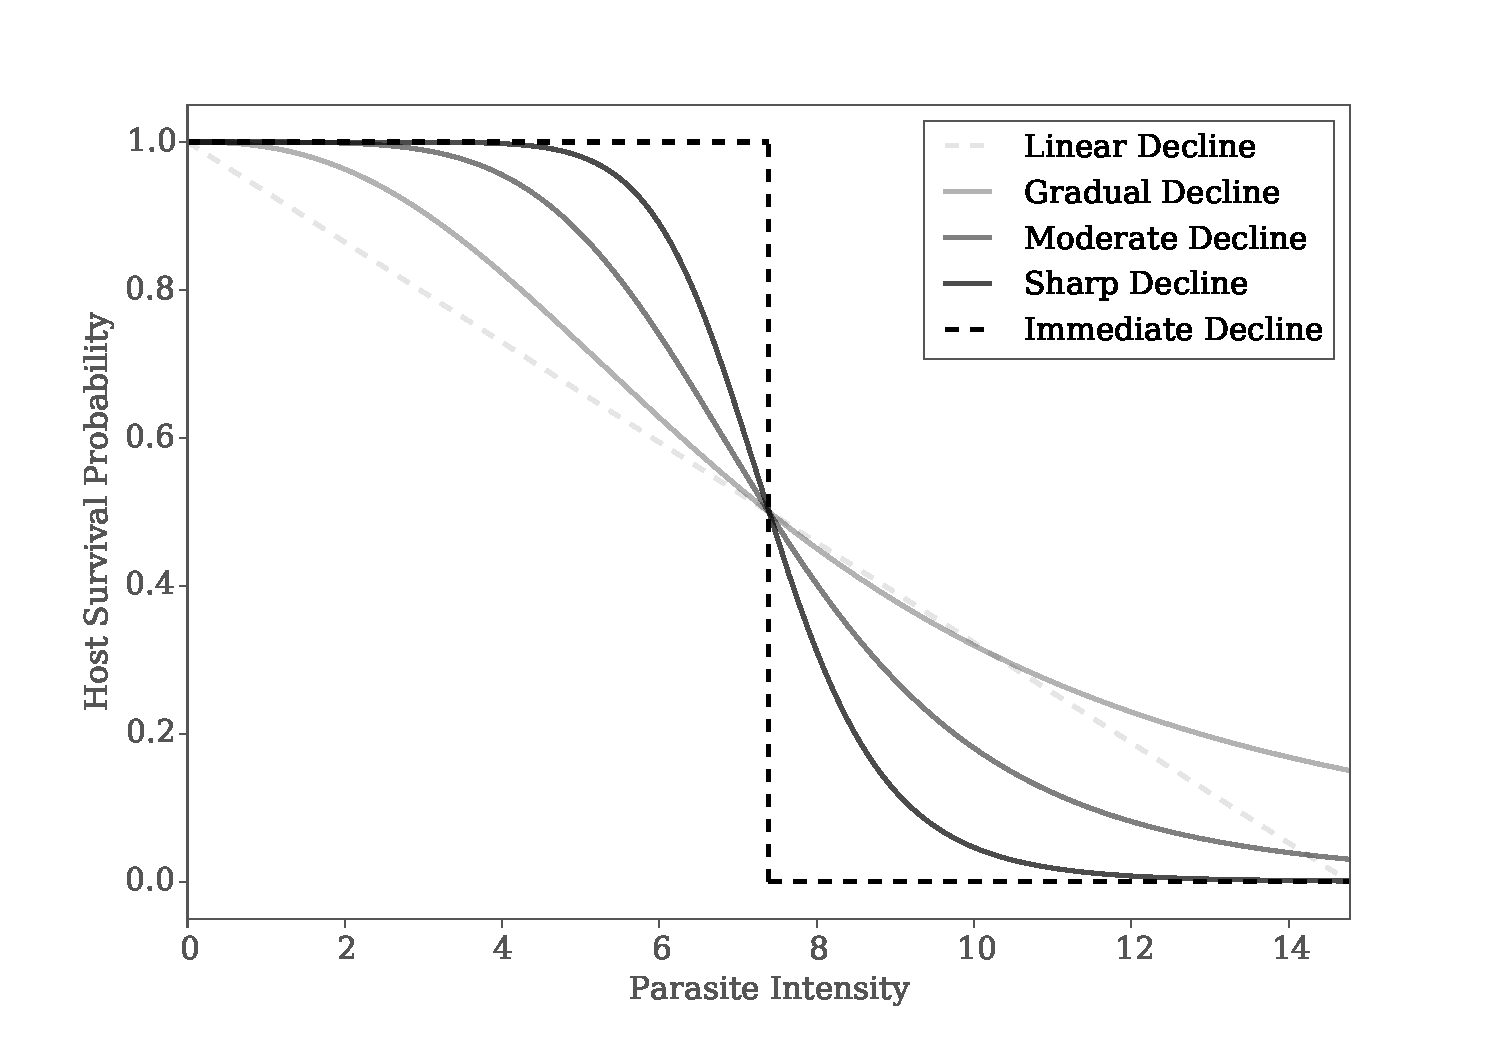
\includegraphics[width=\textwidth]{/Users/mqwilber/Repos/parasite_mortality/results/conceptual_fig.pdf}

    \caption{Five potential shapes for a host-survival functions. PIHM should be easier to detect for steeper host survival functions \citep{Lanciani1989}, but we may expect the bias in the parameter estimates to increase as it becomes increasingly difficult to distinguish between steep survival functions.}
    \label{fig:surv}
\end{figure}

\begin{figure}

    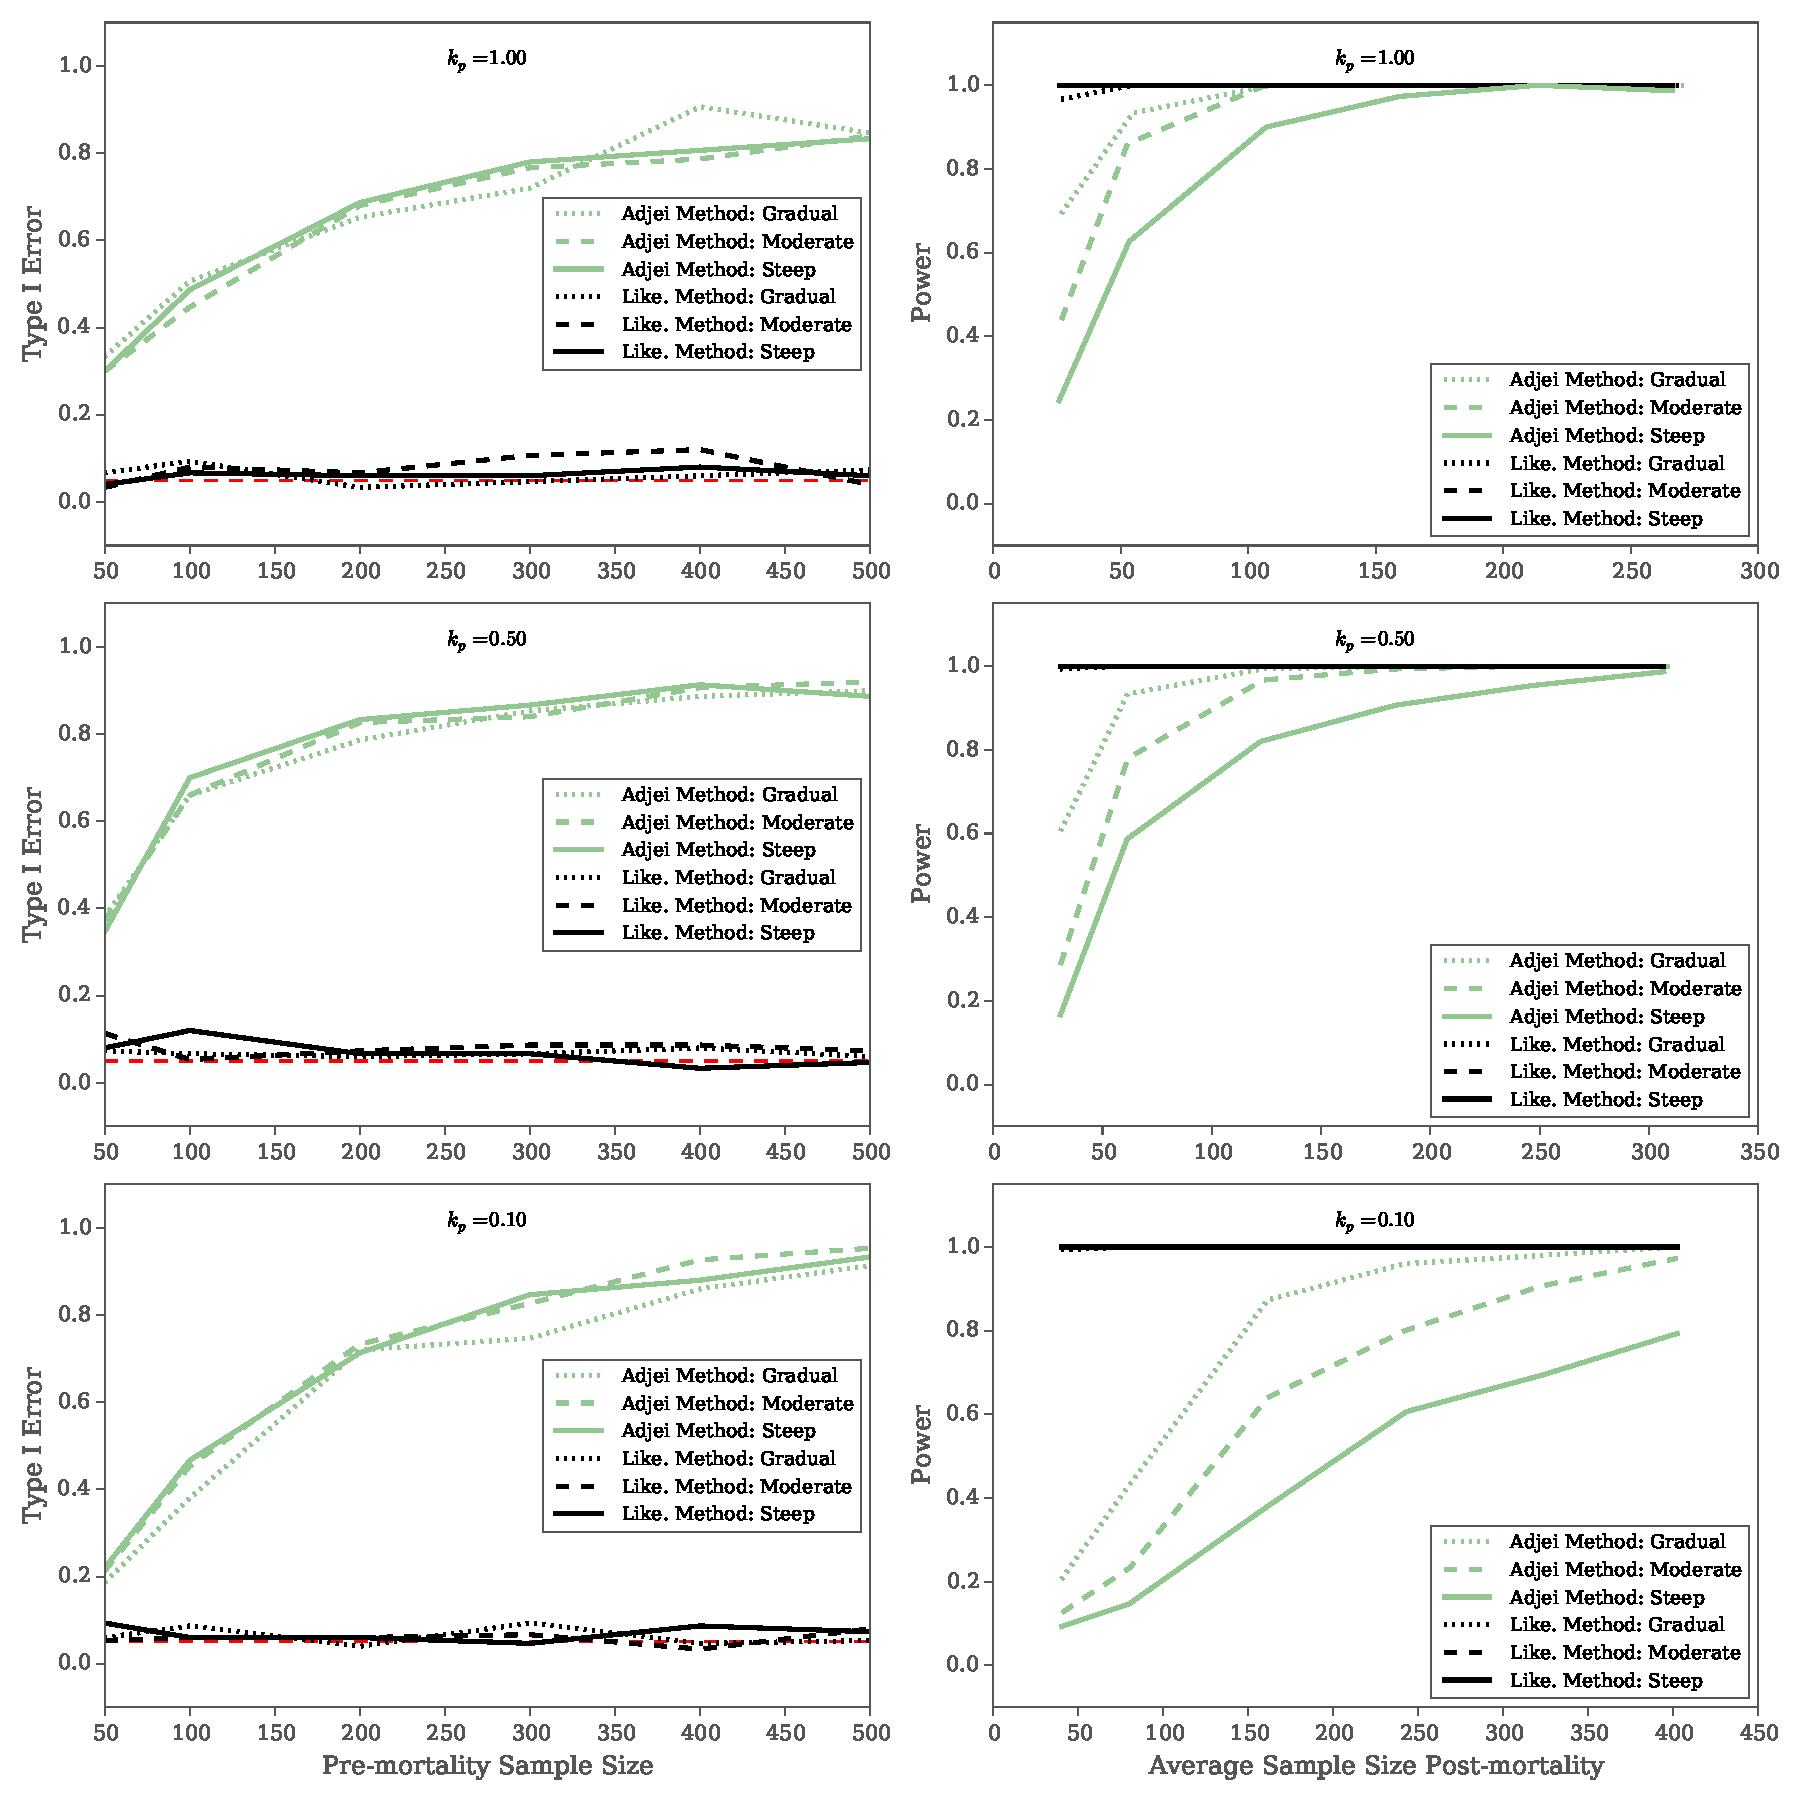
\includegraphics[width=\textwidth]{/Users/mqwilber/Repos/parasite_mortality/results/typeIpower_figure_for_mu10}

    \caption{The Type I error rate and the power of the Likelihood Method (solid line) and the Adjei Method (dashed lines) when $\mu_p = 10$ for various shapes of the host survival function and levels of aggregation $k_p$.  The first column gives the Type I error rate of each method for falsely detecting PIHM when none is present.  The red line gives the the pre-set Type I error rate of $\alpha = 0.05$.  The second column gives the power of a given method to detect PIHM when it is actually occurring. }
    \label{fig:typeI10}

\end{figure}


\begin{figure}

    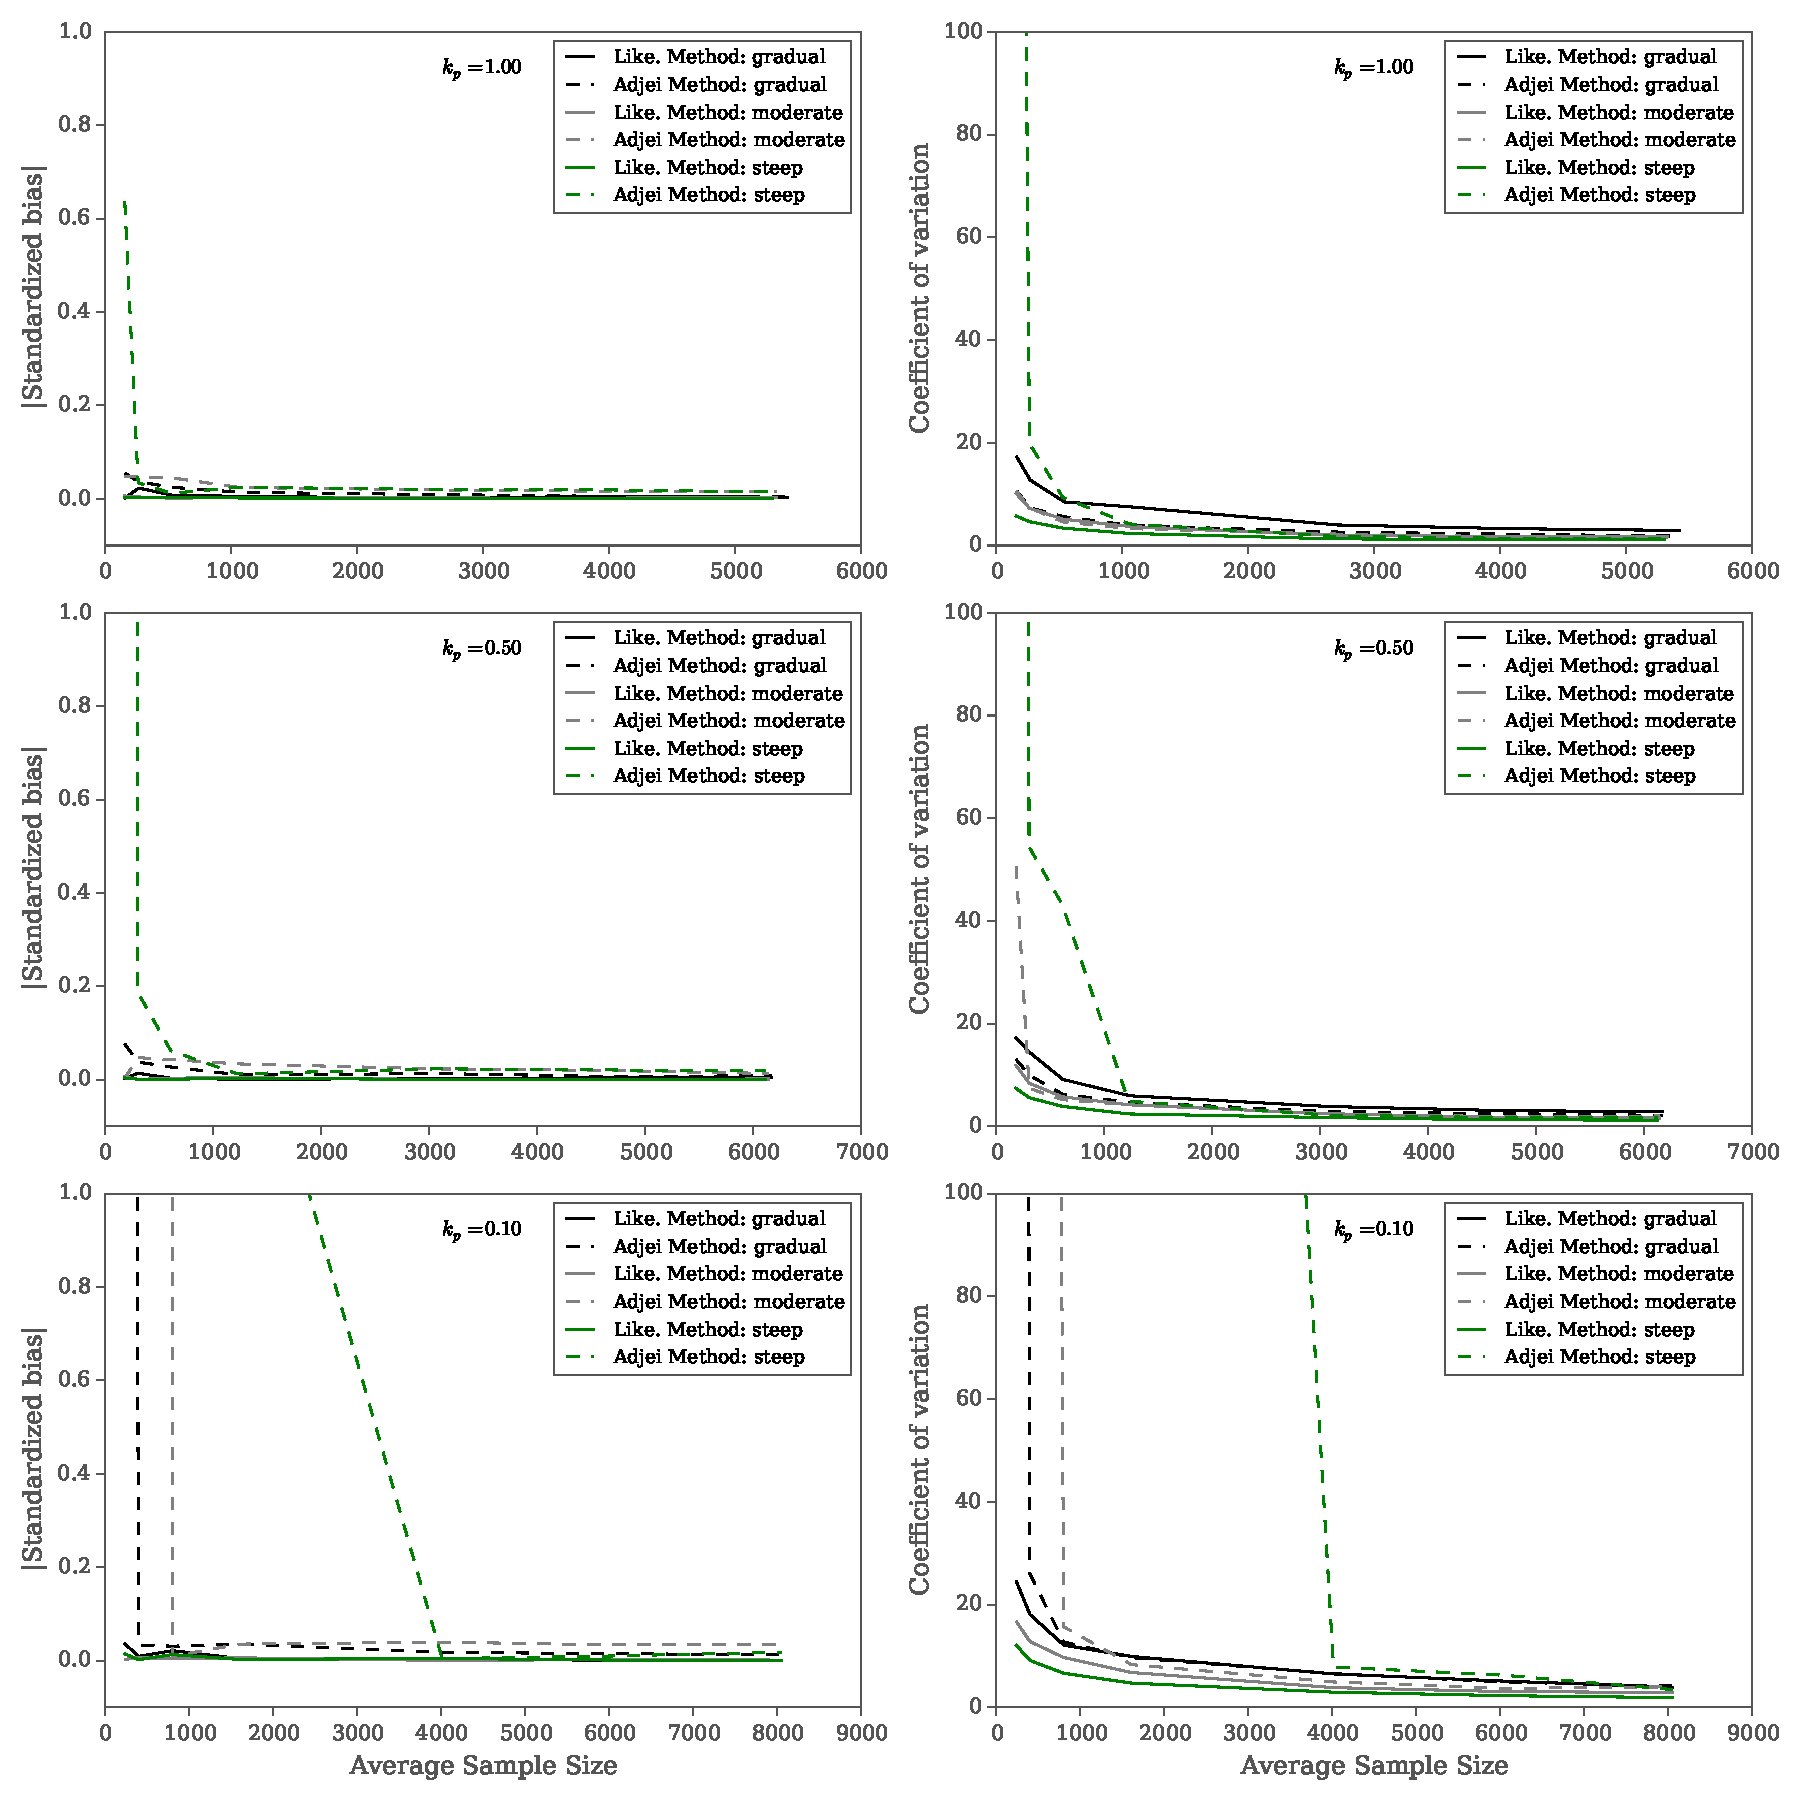
\includegraphics[width=\textwidth]{/Users/mqwilber/Repos/parasite_mortality/results/bais_prec_figure_for_ld50_mu10}

    \caption{The bias and the precision of the Likelihood Method (solid line) and the Adjei Method (dashed lines) when $\mu_p = 10$ for various shapes of the host survival function and levels of aggregation $k_p$ when estimating $LD_{50}$.  The first column gives the bias of each methods $LD_{50}$ estimate over 150 simulations. The second column gives the precision of each methods $LD_{50}$ estimate over 150 simulations.}

    \label{fig:biasld50}

\end{figure}

\begin{figure}

    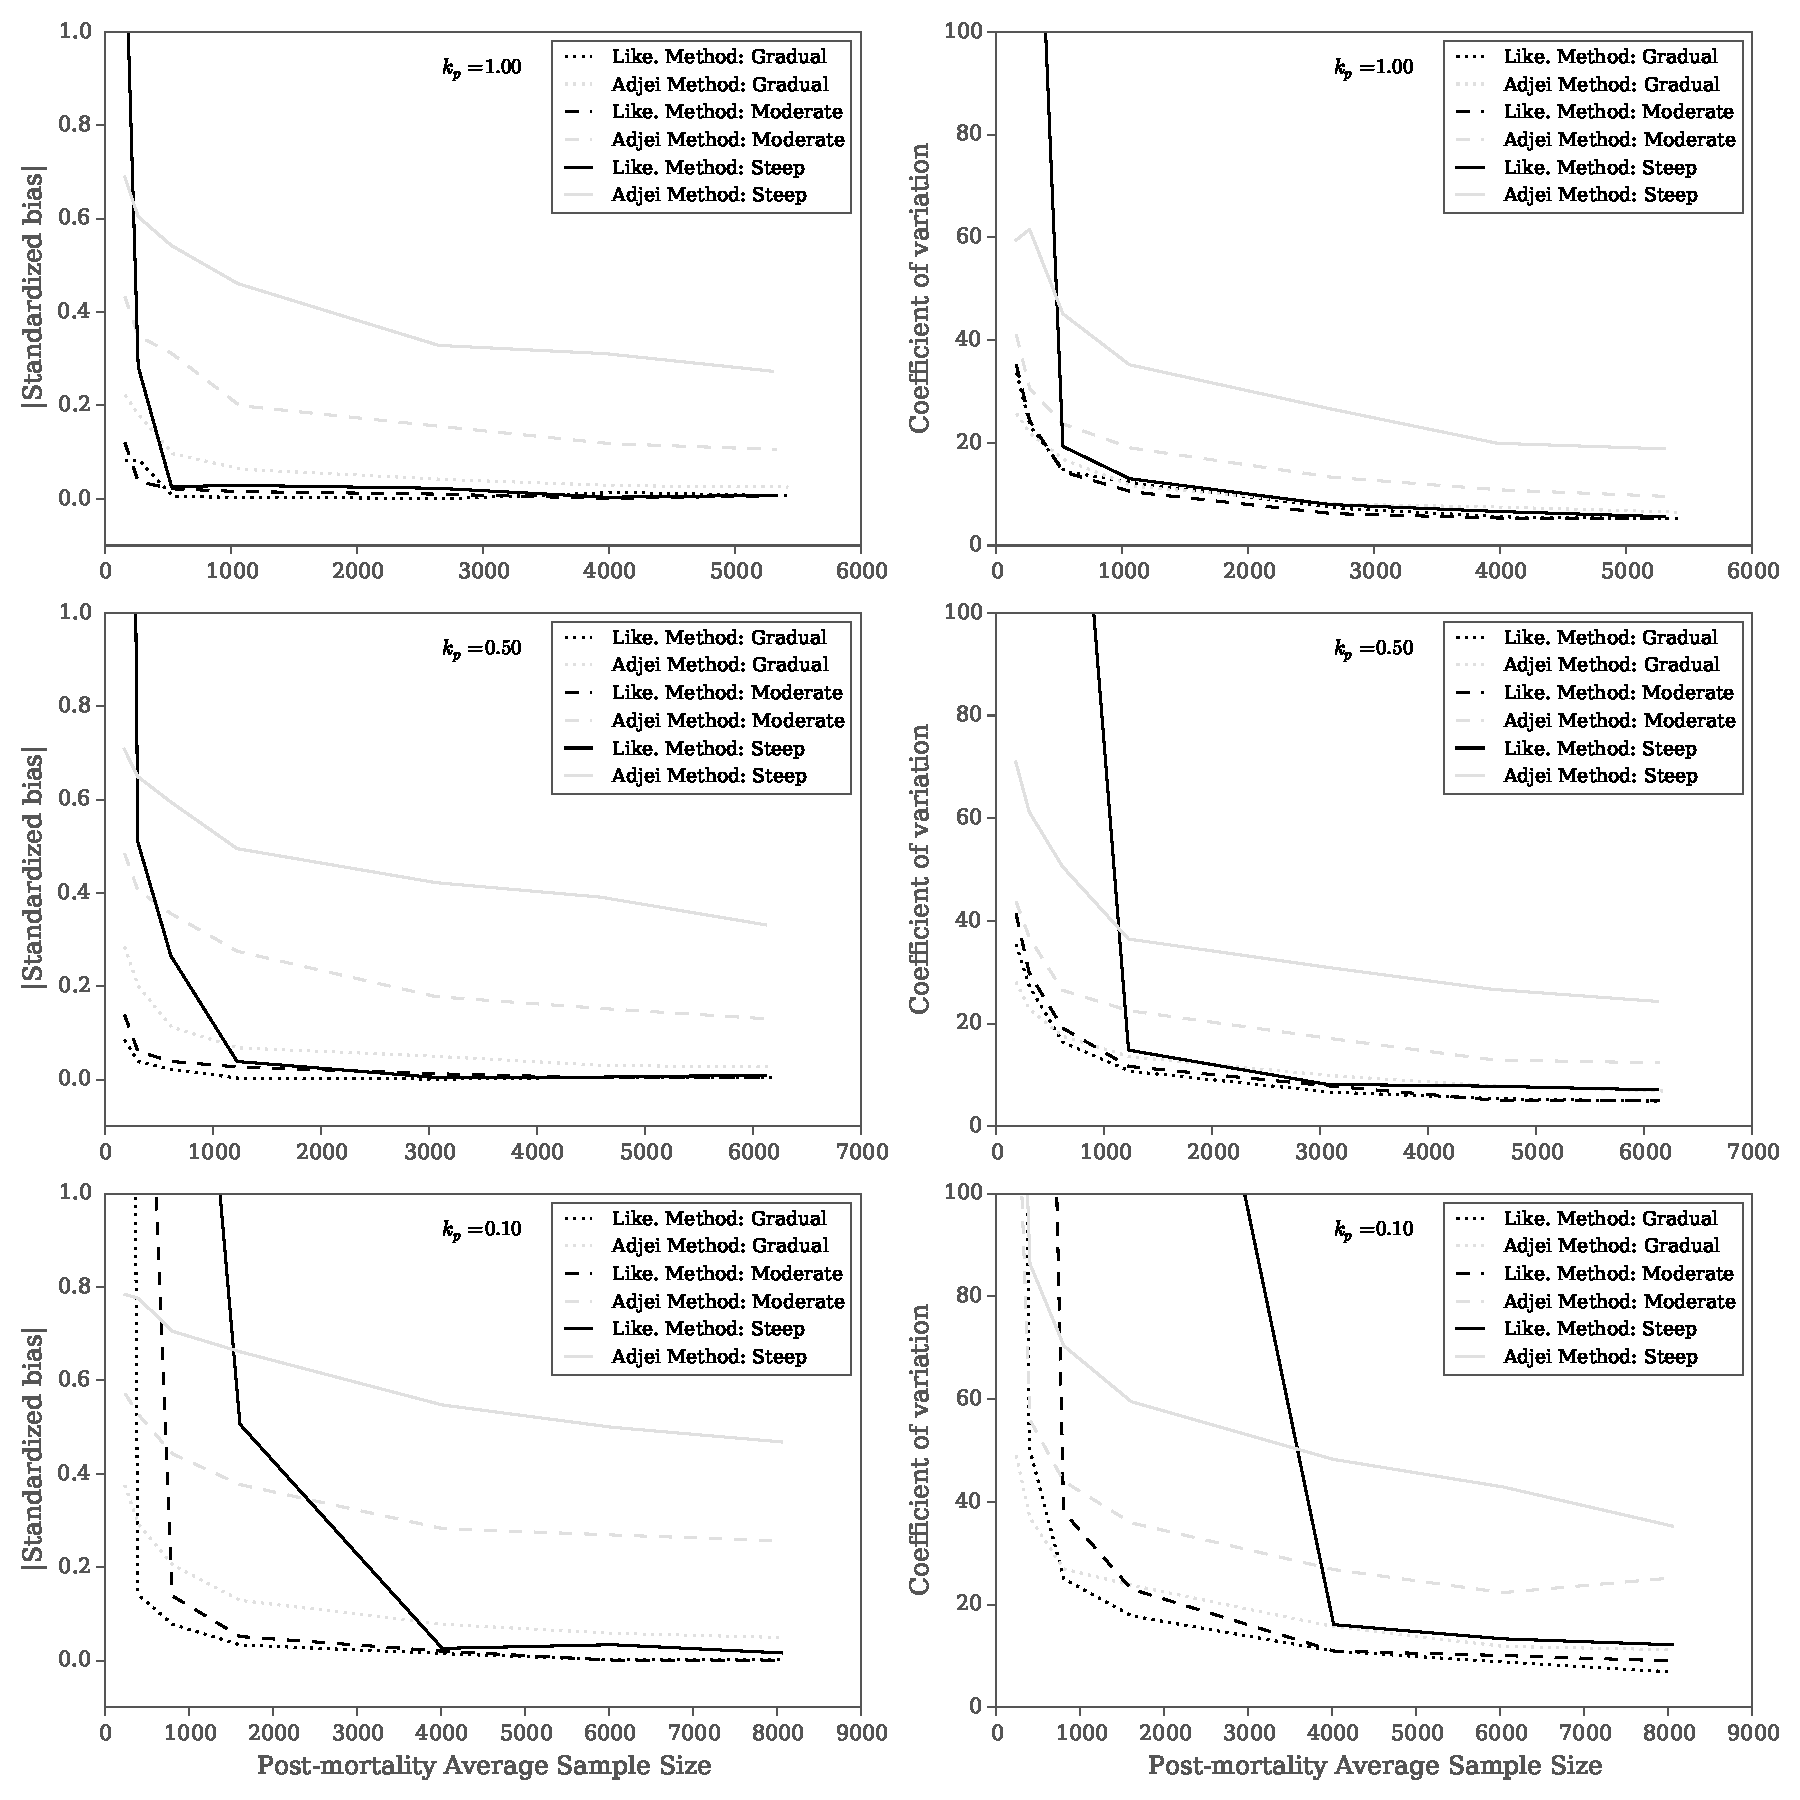
\includegraphics[width=\textwidth]{/Users/mqwilber/Repos/parasite_mortality/results/bais_prec_figure_for_a_mu10}

    \caption{The bias and the precision of the Likelihood Method (solid line) and the Adjei Method (dashed lines) when $\mu_p = 10$ for various shapes of the host survival function and levels of aggregation $k_p$ when estimating the $a$ parameter of the host survival function.  The first column gives the bias of each methods $a$ estimate over 150 simulations. The second column gives the precision of each methods $a$ estimate over 150 simulations.}

    \label{fig:biasa}

\end{figure}




\end{document}

